% Options for packages loaded elsewhere
\PassOptionsToPackage{unicode}{hyperref}
\PassOptionsToPackage{hyphens}{url}
%
\documentclass[
  11pt,
  twocolumn]{article}
\usepackage{amsmath,amssymb}
\usepackage{iftex}
\ifPDFTeX
  \usepackage[T1]{fontenc}
  \usepackage[utf8]{inputenc}
  \usepackage{textcomp} % provide euro and other symbols
\else % if luatex or xetex
  \usepackage{unicode-math} % this also loads fontspec
  \defaultfontfeatures{Scale=MatchLowercase}
  \defaultfontfeatures[\rmfamily]{Ligatures=TeX,Scale=1}
\fi
\usepackage{lmodern}
\ifPDFTeX\else
  % xetex/luatex font selection
\fi
% Use upquote if available, for straight quotes in verbatim environments
\IfFileExists{upquote.sty}{\usepackage{upquote}}{}
\IfFileExists{microtype.sty}{% use microtype if available
  \usepackage[]{microtype}
  \UseMicrotypeSet[protrusion]{basicmath} % disable protrusion for tt fonts
}{}
\makeatletter
\@ifundefined{KOMAClassName}{% if non-KOMA class
  \IfFileExists{parskip.sty}{%
    \usepackage{parskip}
  }{% else
    \setlength{\parindent}{0pt}
    \setlength{\parskip}{6pt plus 2pt minus 1pt}}
}{% if KOMA class
  \KOMAoptions{parskip=half}}
\makeatother
\usepackage{xcolor}
\usepackage[margin=0.1in]{geometry}
\usepackage{graphicx}
\makeatletter
\def\maxwidth{\ifdim\Gin@nat@width>\linewidth\linewidth\else\Gin@nat@width\fi}
\def\maxheight{\ifdim\Gin@nat@height>\textheight\textheight\else\Gin@nat@height\fi}
\makeatother
% Scale images if necessary, so that they will not overflow the page
% margins by default, and it is still possible to overwrite the defaults
% using explicit options in \includegraphics[width, height, ...]{}
\setkeys{Gin}{width=\maxwidth,height=\maxheight,keepaspectratio}
% Set default figure placement to htbp
\makeatletter
\def\fps@figure{htbp}
\makeatother
\setlength{\emergencystretch}{3em} % prevent overfull lines
\providecommand{\tightlist}{%
  \setlength{\itemsep}{0pt}\setlength{\parskip}{0pt}}
\setcounter{secnumdepth}{-\maxdimen} % remove section numbering
% definitions for citeproc citations
\NewDocumentCommand\citeproctext{}{}
\NewDocumentCommand\citeproc{mm}{%
  \begingroup\def\citeproctext{#2}\cite{#1}\endgroup}
\makeatletter
 % allow citations to break across lines
 \let\@cite@ofmt\@firstofone
 % avoid brackets around text for \cite:
 \def\@biblabel#1{}
 \def\@cite#1#2{{#1\if@tempswa , #2\fi}}
\makeatother
\newlength{\cslhangindent}
\setlength{\cslhangindent}{1.5em}
\newlength{\csllabelwidth}
\setlength{\csllabelwidth}{3em}
\newenvironment{CSLReferences}[2] % #1 hanging-indent, #2 entry-spacing
 {\begin{list}{}{%
  \setlength{\itemindent}{0pt}
  \setlength{\leftmargin}{0pt}
  \setlength{\parsep}{0pt}
  % turn on hanging indent if param 1 is 1
  \ifodd #1
   \setlength{\leftmargin}{\cslhangindent}
   \setlength{\itemindent}{-1\cslhangindent}
  \fi
  % set entry spacing
  \setlength{\itemsep}{#2\baselineskip}}}
 {\end{list}}
\usepackage{calc}
\newcommand{\CSLBlock}[1]{\hfill\break#1\hfill\break}
\newcommand{\CSLLeftMargin}[1]{\parbox[t]{\csllabelwidth}{\strut#1\strut}}
\newcommand{\CSLRightInline}[1]{\parbox[t]{\linewidth - \csllabelwidth}{\strut#1\strut}}
\newcommand{\CSLIndent}[1]{\hspace{\cslhangindent}#1}
\usepackage{hyperref}
\usepackage{array}
\usepackage{caption}
\usepackage{graphicx}
\usepackage{multirow}
\usepackage{hhline}
\usepackage{calc}
\usepackage{tabularx}
\usepackage[para,online,flushleft]{threeparttable}
\DeclareMathOperator{\logit}{logit}
\DeclareMathOperator{\var}{var}
\usepackage{float}
\usepackage{booktabs}
\usepackage{longtable}
\usepackage{array}
\usepackage{multirow}
\usepackage{wrapfig}
\usepackage{colortbl}
\usepackage{pdflscape}
\usepackage{tabu}
\usepackage{threeparttable}
\usepackage{threeparttablex}
\usepackage[normalem]{ulem}
\usepackage{makecell}
\usepackage{xcolor}
\ifLuaTeX
  \usepackage{selnolig}  % disable illegal ligatures
\fi
\IfFileExists{bookmark.sty}{\usepackage{bookmark}}{\usepackage{hyperref}}
\IfFileExists{xurl.sty}{\usepackage{xurl}}{} % add URL line breaks if available
\urlstyle{same}
\hypersetup{
  pdftitle={Analysis of Health Survey for England (HSE) 2019},
  pdfauthor={Candidate Numbers Here},
  hidelinks,
  pdfcreator={LaTeX via pandoc}}

\title{Analysis of Health Survey for England (HSE) 2019}
\author{Candidate Numbers Here}
\date{March 14, 2024}

\begin{document}
\maketitle
\begin{abstract}
This report provides an analysis of data related to health, age,
socio-economic factors and lifestyle habits in adults (from the age of
16) from the population in England, derived from the Health Survey for
England 2019. Please note, no generative AI technology was utilized in
the creation of this report or the subsequent data analysis presented
herein. All findings and conclusions are derived from human-driven
methodologies.
\end{abstract}

\pagenumbering{gobble}

\clearpage

\section{Summary}\label{summary}

In England, smoking, ``vaping'' and alcohol consumption are widespread
habits among adults, particularly younger adults. In fact, it is
estimated that around 13.9\% of adults in England identified as
cigarette smokers (\citeproc{ref-1ONS}{ONS 2019a}), and a similar study
found that there were 10.9 alcohol-related deaths per 100,000 people
living in England in 2019 (\citeproc{ref-2ONS}{ONS 2019c}). Thus, it is
crucial to be aware of the predictors and consequences of these habits,
which is the motivation for this analysis.

We conducted this analysis on a subset containing 8,204 adults living in
England (ages 16+), who were interviewed in their homes about their
demographics and their smoking and drinking habits as part of the Health
Survey for England (HSE) 2019. 4,947 of these participants who consented
to an at-home nurse visit had vitals such as blood pressure, weight and
height measured. We investigated which features of a participant are
associated with smoking habits, and which habits are associated with
high blood pressure.

We found alcohol consumption to be the most prevalent lifestyle habit
under investigation. Older males drink the most, especially those aged
65-74. Also, smoking tends to be higher in more deprived areas, while
alcohol consumption is higher in less deprived areas. Socio-economic
factors play an important role in the likelihood of smoking. On average,
females are 25\% less likely to be smokers than males. Ethnicity also
play a great role, being Black or Asian decreases the likelihood of
smoking by over 70\% and 65\%, respectively. Females are much less
likely to experience hypertension in comparison to males. However,
systolic blood pressure levels are positively correlated with age and
how often the respondent drinks alcohol, regardless of gender.

\subsection{Introduction}\label{introduction}

The mechanisms which drive lifestyle habits are part of a complex and
ever-changing field in behavioural psychology. What is known, however,
is that such habits are driven by cues and cravings
(\citeproc{ref-SmokeCue}{Anastasia Droungas 1995};
\citeproc{ref-DrinkCue}{Kambouropoulos 2009}). The HSE 2019 captures
demographic and socioeconomic characteristics that have the potential to
make such cues more visible and cravings harder to resist. For example,
living in a region where smoking is more prevalent or not having a
husband/wife for an accountability partner to help you quit or resist
these habits (\citeproc{ref-AccountPartner}{ONS 2019b}).

In this report, we will use weighting variables to estimate prevalence
of cigarette, e-cig, and alcohol users in our population, and compare it
with the larger population of adults in England. We will then attempt to
identify associations with a participants current smoking status,
explore whether predictive modelling can be used to identify smokers
with a high accuracy, and investigate which lifestyle habits are
associated with increased values of systolic blood pressure. Such an
understanding would be crucial in enabling healthcare providers to
implement preventative care for people at risk of developing
hypertension.

\section{Methodology}\label{methodology}

\subsection{Exploratory Analysis}\label{exploratory-analysis}

The full HSE 2019 cross-sectional data set contains 10,299 observations
across thousands of variables (\citeproc{ref-Main}{NatCen Social
Research and Health 2019}), but we only studied patients over the age of
16 among key variables. Our subset includes 8,204 participants and 19
variables, which are described in Table \ref{tab:output-var-table}.

\begin{table}
\centering
\caption{\label{tab:outputvartable}Summary of the analysis variables used in our report. (D) indicates that a variable was derived.\label{tab:output-var-table}}
\centering
\fontsize{8}{10}\selectfont
\begin{tabular}[t]{>{\raggedright\arraybackslash}p{7em}|>{\raggedright\arraybackslash}p{11em}|l}
\hline
\textbf{Variable} & \textbf{Definition} & \textbf{Notation}\\
\hline
SerialA & Respondent serial number & ID\\
\hline
wt\_int & Weight of observation & w\\
\hline
Sex & Respondent sex (M/F) & $s$\\
\hline
(D) Age35g & Respondent age grouped in 5 year bands for 16+ & $a^{(5)}$\\
\hline
(D) ag16g10 & Respondent age grouped in 10 year bands for 16+ & $a^{(10)}$\\
\hline
(D) topqual2 & Highest level qualification & $t$\\
\hline
(D) marstatD & Marital status & $ms$\\
\hline
(D) qimd19 & IMD score (a measure of deprivation) & $q$\\
\hline
(D) urban14b & Level of rurality & $u$\\
\hline
(D) origin2 & Grouped ethnic category & $o$\\
\hline
(D) cigdyal\_19 & $\#$ of cigarettes smoked per day & $n^{cig}$\\
\hline
(D) cigsta3\_19 & Smoking status (Reg / Ex-Reg / Never-Reg) & $cig$\\
\hline
(D) NDPNow\_19 & Use of E-cigarettes and or NDPs & $ndp$\\
\hline
(D) DrinkYN\_19 & Alcohol consumed in the last 12 months & $alc$\\
\hline
dnoft\_19 & Frequency of alcohol consumed in the last 12 months (grouped) & f\\
\hline
(D) d7many3\_19 & $\#$ of days alcohol was consumed in the last week & $n^{alc}$\\
\hline
(D) GOR1 & Government region office number & $g$\\
\hline
(D) BMIval & Valid BMI measurement (weight estimated if $\>$ 130kg) & $bmi$\\
\hline
(D) omsysval & Valid mean systolic blood pressure & $sbp$\\
\hline
(D) smoking\_status & Current smoking status (binary) & $S$\\
\hline
(D) estim\_age & Estimated age & $a$\\
\hline
\end{tabular}
\end{table}

\subsubsection{Duplicates}\label{duplicates}

We found 36 pairs of observations with exactly equal variables
(excluding ID variables and lab measurements), but we did not remove
these from our analysis because the supporting documentation didn't
state a protocol for repeated visits. We assumed these were genuine
observations from different participants and thus included them in our
dataset. However, there were 3 pairs of observations that had duplicate
lab variables also. Due to the high precision of measurements, we
believed these to be true duplicates and removed one observation from
each of the three pairs, resulting in a dataset of 8201 observations.

\subsubsection{Dichotomy of Factors}\label{dichotomy-of-factors}

All variables were originally coded as numeric in our dataset, so we
recoded these to factor variables accordingly. Some of the variables
used for analysis were dichotomised by us for easier interpretation. We
coded a binary variable indicating current smoking status, which will
serve as a response variable. Also, we dichotomised urbanity into two
levels being `Rural' and `Urban', and finally marital status into
`Married' and `Not Married'. We grouped respondents' level of education
into `Higher Education', `Further Education', `A-Level equiv.', `GCSE
equiv.', `No qualification' and `Foreign/other', and we grouped alcohol
frequency into ``Frequent'', ``Occasional'' and ``Rarely'' based on the
response to the question ``How often did you consume alcohol in the last
12 months?''.

\subsubsection{Missingness}\label{missingness}

\begin{table}
\centering
\caption{\label{tab:outputnatable}Missing values in the training dataset\label{tab:output-na-table}}
\centering
\fontsize{9}{11}\selectfont
\begin{tabular}[t]{l|r|l}
\hline
\textbf{Variable} & \textbf{Missing Values} & \textbf{\% Missing}\\
\hline
omsysval & 4036 & 61.5\%\\
\hline
BMIVal & 1519 & 23.2\%\\
\hline
dnoft\_19 & 1496 & 22.8\%\\
\hline
cigdyal\_19 & 57 & 0.869\%\\
\hline
cigsta3\_19 & 56 & 0.854\%\\
\hline
NDPNow\_19 & 53 & 0.808\%\\
\hline
d7many3\_19 & 52 & 0.793\%\\
\hline
drinkYN\_19 & 51 & 0.777\%\\
\hline
topqual2 & 46 & 0.701\%\\
\hline
origin2 & 29 & 0.442\%\\
\hline
marstatD & 1 & 0.0152\%\\
\hline
\end{tabular}
\end{table}

There is significant missingness in the lab values, as shown in Table
\ref{tab:output-na-table}. These can be explained by the fact additional
consent was needed from the participant to allow a nurse visit. One
variable with a substantial amount of data missing was the frequency of
drinking in the last 12 months, which due to the retrospective and
sensitive nature of the question could be explained by either recall
bias or a participant's refusal to answer. As a result, we decided to
remove this variable from analysis in favour of a binary variable which
simply states whether the respondent has drunk alcohol in the last 12
months. Education level, marital status and ethnicity are the only
socioeconomic variables with any missing entries, with 46 observations
(0.701\% of the data) missing at least one of the three. These are not
necessary for identifiability and as they are sensitive, we do not
expect every participant to answer these questions. Therefore, we did
not remove these observations.

\subsubsection{Outliers and Data Issues}\label{outliers-and-data-issues}

We attempted to determine whether the two lab measurement variables
contained potential outliers, and as can be seen in Figure
\ref{fig:output-distribution-plots}, there were many outliers for BMI.
We note that this used self-estimated weight from the participant in the
calculation when it exceeded 130kg. Additionally, weight measurements
were taken in inconsistent environments such as on different flooring in
the participants' homes which will impact measurement accuracy. We
believed this could have explained the extremely high BMI values in the
range of 54.82 to 73.49. We coded such values as missing in the analysis
dataset, but kept the observation.

The readings for systolic blood pressure were collected by taking an
average of three readings, each five minutes apart, performed by a
trained nurse who had to declare each reading to be valid. For this
reason, it seemed highly unlikely that these readings were mistakes, and
so we included them in our analysis. The measurement device used has
been validated for use in this environment (\citeproc{ref-Omron}{Yechiam
Ostchega PhD 2009}). We did, however, note that values of systolic blood
pressure that were this consistently high (\textgreater140mmHg) were
indicators for hypertensive crisis, and so a part of our population may
have serious underlying health conditions that could affect the
generalisability of our findings (\citeproc{ref-heart}{Association
2023}).

\begin{figure}[H]
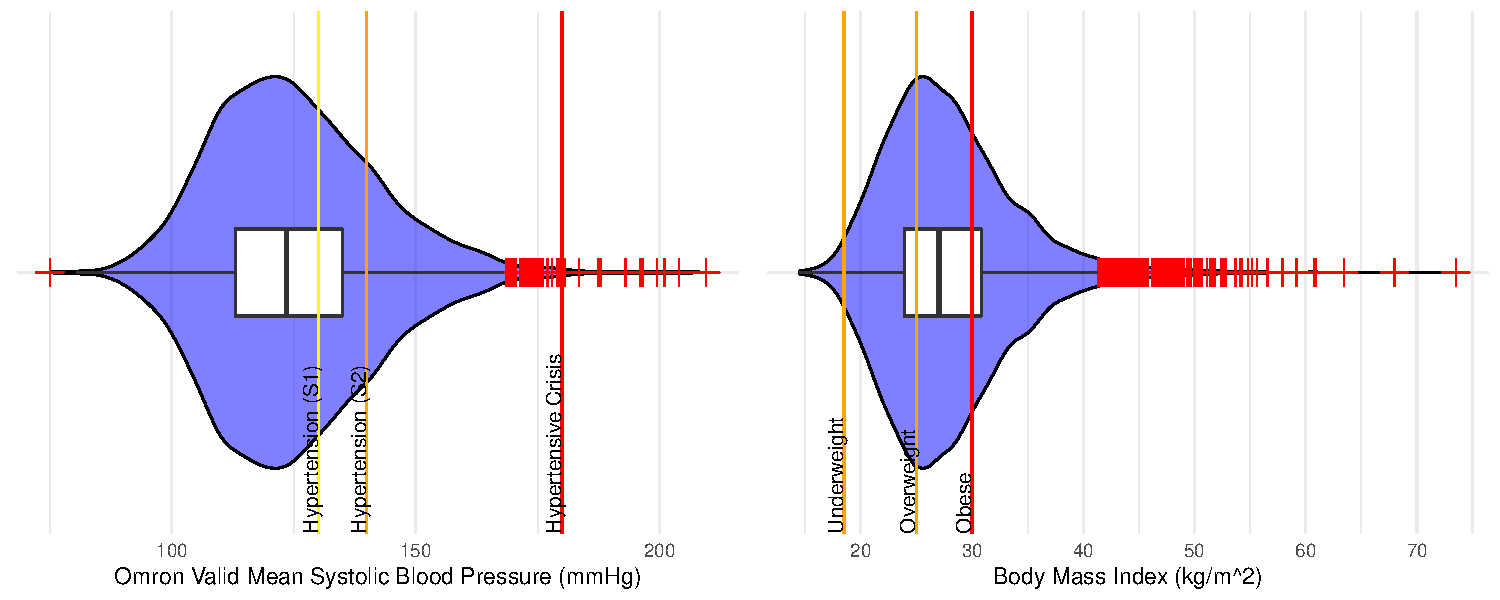
\includegraphics{Coursework_files/figure-latex/output-distribution-plots-1} \caption{Distribution of BMI and Mean Systolic Blood Pressure}\label{fig:output-distribution-plots}
\end{figure}

\section{Analysis}\label{analysis}

\subsubsection{What is the prevelence of drinking, smoking and E-cig
usage?}\label{what-is-the-prevelence-of-drinking-smoking-and-e-cig-usage}

To calculate the prevalence of these three habits we assumed each of the
\(n\) observations, \(x_1,…,x_n\) , to be independent, identically
distributed (iid) random variables (RVs) where
\(x_i \sim Bern(p)\, \forall i=1,…,n\) and \(p\) denotes the probability
of a habit being present for the given observation.

We used the household-level weighting variable to calculate a weighted
Maximum Likelihood Estimate (MLE) of \(p\). That is, letting \(w_i\)
denote the weight of the \(i^{th}\) observation, we altered the standard
likelihood function of a Bernoulli distribution as below:
\[L(p|\textbf{x}) = \prod_{i = 1}^{n} (p^{x_i}(1-p)^{1-x_i})^{w_i}\]
From this, we calculated our weighted MLE as
\(\widehat{p} = \frac{\sum_{i=1}^{n} x_iw_i}{\sum_{i=1}^{n} w_i}\). It
can also be shown that the MLE has variance given by
\(\mathop{\mathrm{var}}(\widehat{p})=\frac{p(1-p)}{\sum_{i=1}^{n}w_i}\),
which we estimated using \(\widehat{p}\). We used large sample
properties of the MLE to get a normal approximation and estimated 95\%
confidence intervals for each habit, which are shown in Table
\ref{tab:output-estimates-table}.

\begin{table}
\centering
\caption{\label{tab:outputestimatestable}Estimates and 95\% Confidence Intervals for \% of Population\label{tab:output-estimates-table}}
\centering
\fontsize{9}{11}\selectfont
\begin{tabular}[t]{l|l|l}
\hline
\textbf{Habit} & \textbf{Estimate} & \textbf{C.I.}\\
\hline
Drinking & 80.4\% & (79.5\%, 81.2\%)\\
\hline
Smoking & 16.5\% & (15.7\%, 17.3\%)\\
\hline
Smoking E-cigarettes & 4.28\% & (3.84\%, 4.72\%)\\
\hline
\end{tabular}
\end{table}

We found that the usage of e-cigarette usage among adults is relatively
low, making it challenging to dissect any significant trends within the
data. However, since drinking and smoking were so prevalent among the
respondents, we had sufficient data to identify any potential trends
within sub-categories of individuals.

Next, we worked to uncover factors that have possible associations with
smoking prevalence. We started with the demographic factors of age and
gender, plotting the smoking prevalence across combinations of these
groups to identify any patterns. Figure \ref{fig:output-prevelance-plot}
suggests a negative correlation between age and the proportion of
current cigarette smokers, across both genders. Interestingly, the
proportion of males who quit smoking in later-life was much greater than
that of females (75yrs+; M: 50\%, F: 31\%).

\begin{figure}[H]
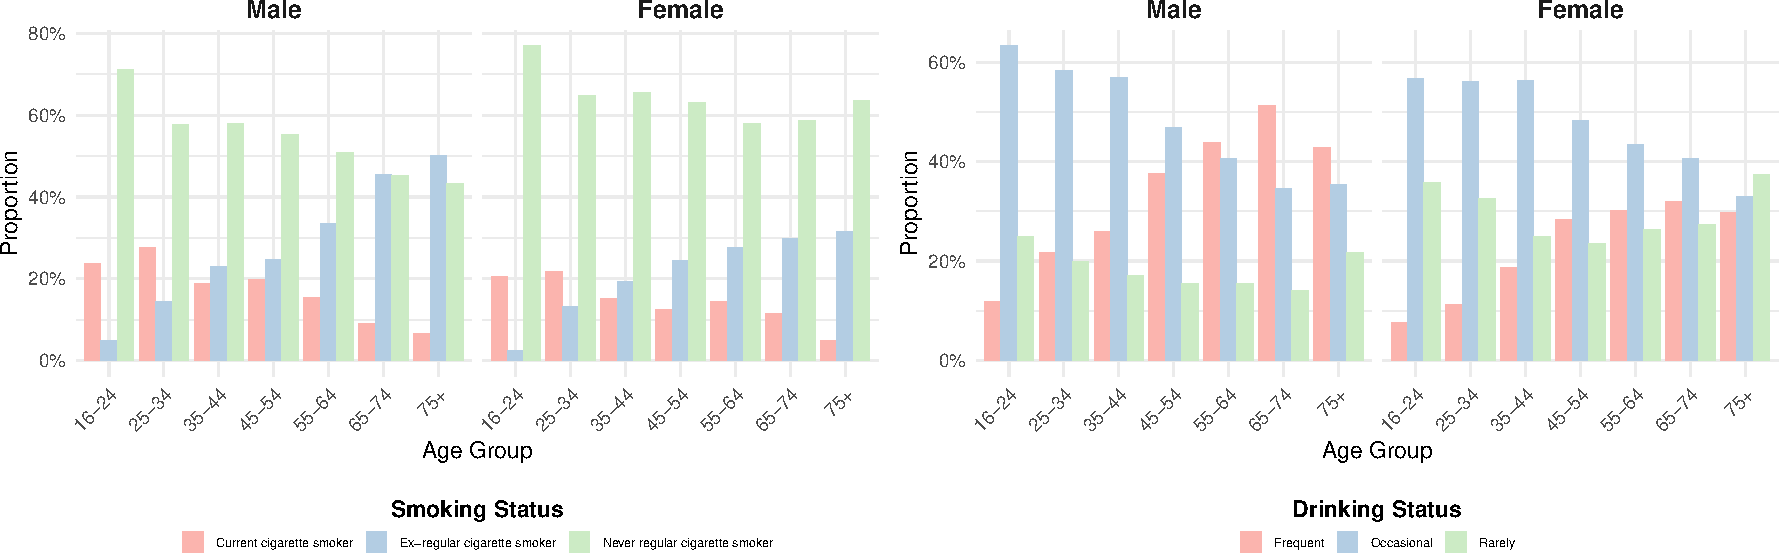
\includegraphics{Coursework_files/figure-latex/output-smoking-drinking-age-plot-1} \caption{Smoking and drinking status proportions by age group and gender}\label{fig:output-smoking-drinking-age-plot}
\end{figure}

\begin{figure}[H]
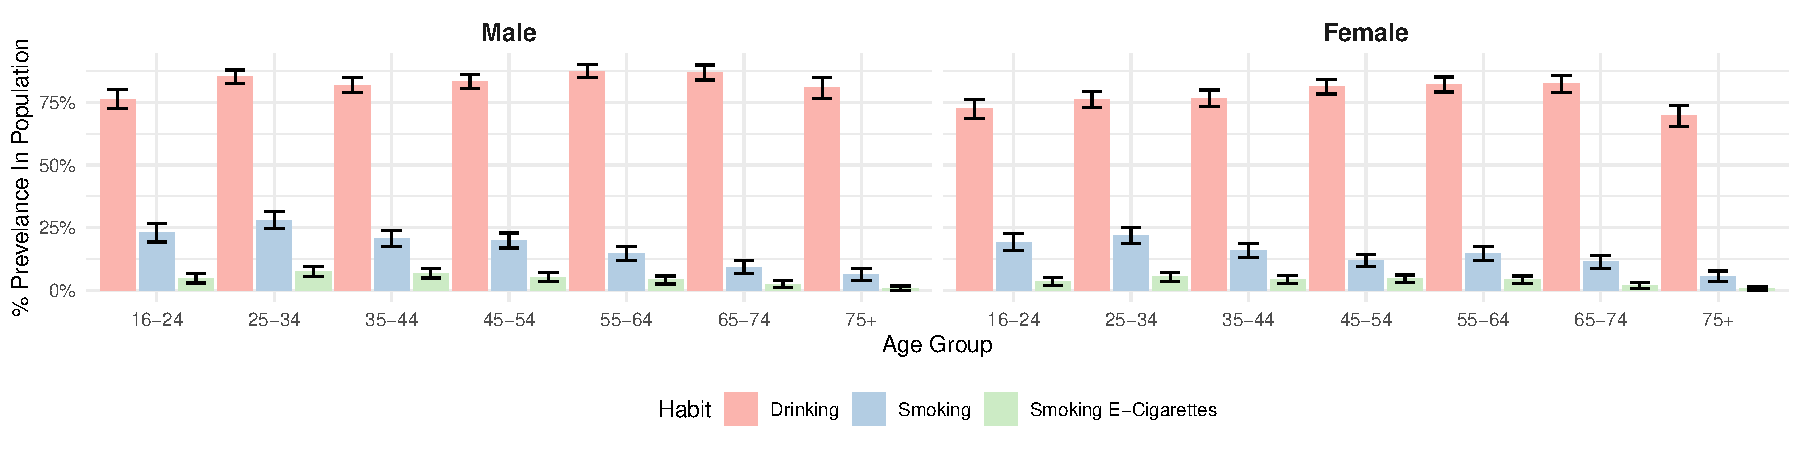
\includegraphics{Coursework_files/figure-latex/output-prevelance-plot-1} \caption{Estimation of the prevelance of habits by age group and gender.}\label{fig:output-prevelance-plot}
\end{figure}

We found males demonstrate a higher prevalence of drinking across nearly
all demographic categories in comparison to females. We observed a
positive correlation between smoking and deprivation levels, with
25.76\% of individuals in the most deprived quintile being smokers, a
significant increase when compared to 9.33\% in the least deprived.

\subsubsection{How is smoking associated with socioeconomic factors and
age?}\label{how-is-smoking-associated-with-socioeconomic-factors-and-age}

We reserved 80\% of our data to train the model, and used the remaining
20\% to test the model, which was made possible due to the large size of
our dataset. The training set contained 6561 observations and the test
set contained 1640. Table \ref{tab:output-testtrain-table} summarises
the key variables between the test and train dataset to illustrate that
both are representative of the whole dataset. This reduced the risk of
overfitting and allowed us to test the predictive power of each model we
proposed.

\begin{table}
\centering
\caption{\label{tab:outputtesttraintable}Comparison of the characteristics of the training set compared with the test set.\label{tab:output-testtrain-table}}
\centering
\fontsize{10}{12}\selectfont
\begin{tabular}[t]{l|l|l}
\hline
\multicolumn{1}{c|}{ } & \multicolumn{2}{c}{Proportion (\%)} \\
\cline{2-3}
\textbf{Variable:Label} & \textbf{Test} & \textbf{Train}\\
\hline
Sex:Male & 43.5 & 45.1\\
\hline
Sex:Female & 56.5 & 54.8\\
\hline
 &  \vphantom{3} & \\
\hline
topqual2:No qualification & 19.7 & 19.8\\
\hline
topqual2:GCSE equiv. & 21.2 & 20.9\\
\hline
topqual2:A-Level equiv. & 14.0 & 13.4\\
\hline
topqual2:Further Education & 28.5 & 28.4\\
\hline
topqual2:Higher Education & 15.9 & 16.1\\
\hline
topqual2:Foreign/Other & 0.7 & 1.3\\
\hline
 &  \vphantom{2} & \\
\hline
marstatD:Married & 55.4 & 51.9\\
\hline
marstatD:Not Married & 44.6 & 48.1\\
\hline
 &  \vphantom{1} & \\
\hline
urban14b:Urban & 80.3 & 81.4\\
\hline
urban14b:Not Urban & 19.7 & 18.6\\
\hline
 &  & \\
\hline
origin2:White & 85.9 & 85.8\\
\hline
origin2:Black & 3.1 & 2.9\\
\hline
origin2:Asian & 8.8 & 8.7\\
\hline
origin2:Multiple & 1.4 & 1.7\\
\hline
origin2:Other & 0.8 & 0.9\\
\hline
\textbf{} & \textbf{Mean} & \textbf{Mean}\\
\hline
Age(Estimated) & 51.2 & 51.0\\
\hline
\end{tabular}
\end{table}

To develop a predictive model for identifying smokers, we used the
binary variable for current smoking status as a response, with various
socioeconomic and demographic factors as predictors. These were selected
based on the associations suggested by our prior analysis.

Under the assumption that the age of participants were approximately
uniformly distributed within their respective age bands, we defined the
estimated age of the \(i^{th}\) observation as the midpoint of the
participants respective 5-year age group (taking the estimation of the
90+ category as 92.5), denoted \(a_i\). We found that age may represent
a somewhat quadratic effect on the probability of smoking, leading us to
include a \(a_i^2\) term in our model. A comparison of these models are
summarised in Table \ref{tab:output-model-selection-table}.

We selected the model based on AIC, which enabled us to balance model
complexity and model fit (quantified by likelihood), which further
reduced the risk of overfitting. This model is:

\[\text{logit}(\mu_i) \sim \beta_0 + \beta_1a + \beta_2a^2 + \beta_3q + \alpha^{ms}_j + \alpha^{u}_k + \alpha^{o}_l + \alpha^{t}_m + \alpha^{s}_n \\
\text{where } j \in \{\text{Married, Not Married}\}, k \in \{\text{Urban, Not Urban}\}, l \in \{\text{White,}\ldots\text{,Black}\}, n \in \{\text{Male, Female\} and}\  m \in \{\text{Higher Education,}\ldots\text{, No qualification}\}\].

\begin{table}
\centering
\caption{\label{tab:outputmodelselectiontable}Comparison of selected model evaluations, wherein $\eta_i = \text{logit}(\mu_i)$, and Acc. refers to the model accuracy on test data.\label{tab:output-model-selection-table}}
\centering
\fontsize{8}{10}\selectfont
\begin{tabular}[t]{>{\raggedright\arraybackslash}p{7em}|r|r|r|r|r}
\hline
\multicolumn{3}{c|}{ } & \multicolumn{2}{c|}{RMSE} & \multicolumn{1}{c}{ } \\
\cline{4-5}
\textbf{Model} & \textbf{AIC} & \textbf{AUC} & \textbf{Train} & \textbf{Test} & \textbf{Acc.}\\
\hline
$\eta_i \sim a_i + a_i^2 + ms_i + q_i + u_i + o_i + t_i + s_i$ & 4987.3 & 0.759 & 0.342 & 0.324 & 0.861\\
\hline
$\eta_i \sim a_i + ms_i + q_i + u_i + o_i + t_i + s_i$ & 5036.4 & 0.740 & 0.343 & 0.327 & 0.861\\
\hline
$\eta_i \sim a_i^{(5)} + ms_i + q_i + u_i + o_i + t_i + s_i$ & 4994.3 & 0.759 & 0.341 & 0.325 & 0.861\\
\hline
$\eta_i \sim a_i^{(10)} + ms_i + q_i + u_i + o_i + t_i + s_i$ & 5005.9 & 0.753 & 0.342 & 0.324 & 0.860\\
\hline
\end{tabular}
\end{table}

To evaluate the predictive performance of our final model using our test
data, Figure 4 demonstrates the predicted probability of each
`probability bin' against the mean actual outcomes. As we can see the
calibration curve closely follows the line \(y = x\), which is
indicative of a well-calibrated model.

This model doesn't predict high values due to the low prevalence of
smoking within the population. The highest likelihood our model predicts
is 63.75\% All results should be interpreted with the population average
in mind, which is \textasciitilde16.5\%. For example, if the model
predicts the likelihood of an individual being a smoker at 33\%, said
individual is twice as more likely to be a smoker than the average. This
effect can be seen in the following calibration chart.

\begin{figure}[H]

{\centering 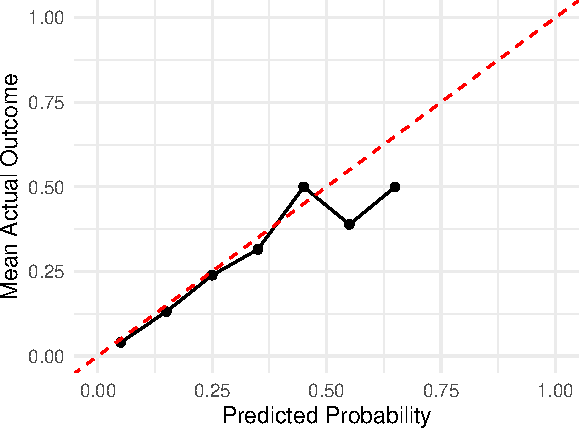
\includegraphics{Coursework_files/figure-latex/output-calibration-chart-1} 

}

\caption{Calibration chart for Binomial model}\label{fig:output-calibration-chart}
\end{figure}

\begin{figure}[H]
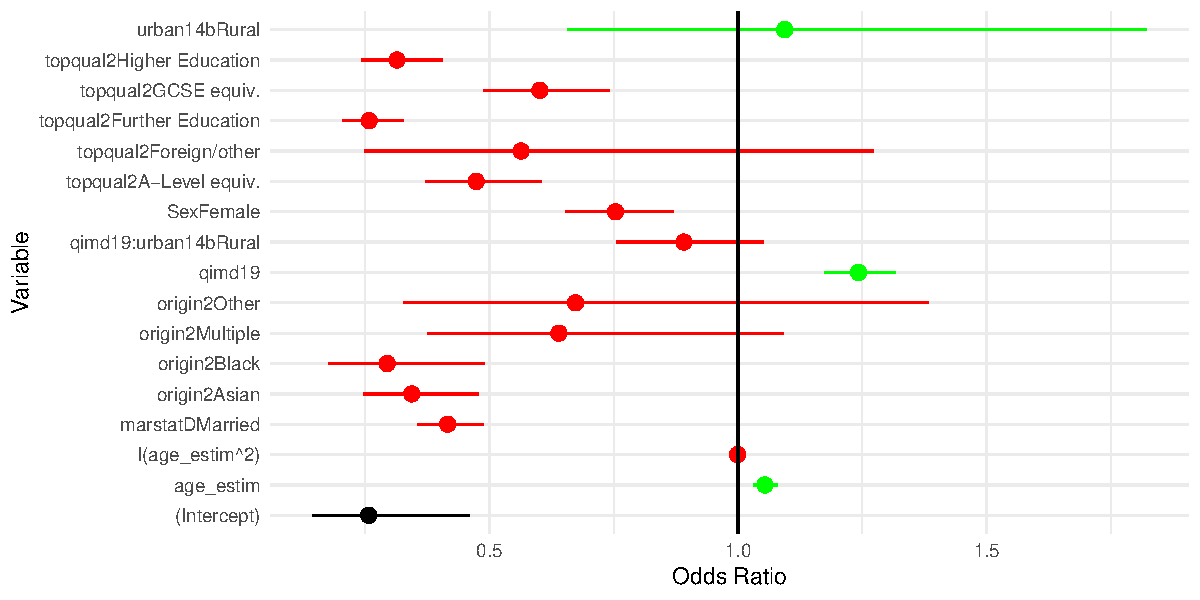
\includegraphics{Coursework_files/figure-latex/output-forest-plot-1} \caption{Forest plot of Odds Ratios for the binomial model}\label{fig:output-forest-plot}
\end{figure}

\subsubsection{Which lifestyle habits are associated with systolic blood
pressure?}\label{which-lifestyle-habits-are-associated-with-systolic-blood-pressure}

We chose to model the systolic blood pressure (BP) using the
Inverse-Normal distribution with a \(1/\mu_i^2\) link function. As we
noted before this variable has a lot of outliers, is right-skewed and
strictly positive, making this distribution a good choice. We also
tested a Log-Normal distribution, a Normal distribution with identity
link and a Gamma distribution with an inverse link but found that the
Inverse-Normal distribution was able to account for the higher values of
BP the best when we compared the Q-Q plots. The data we used to fit this
model was the same training data set as the Binomial model. We filtered
out \emph{NA} values of BMI and BP as we only want to consider
respondents that had lab measurements taken, leaving us with 2960
observations.

We studied the relationship between both age and BMI with BP, shown in
Figure \ref{fig:output-relationship-plots}. There was a quadratic
relationship between BMI and BP so we decided to include a \(bmi^2\)
term in our model. To account for possible dependencies between
variables in the data, we tried fitting models with a combination of
different interaction terms and found three that were likely
significant. These were between BMI \& Age
(\citeproc{ref-AgeBMI}{Medicine 2017}), BMI \& gender
(\citeproc{ref-SexBMI}{K. et al. 2019}) and Age \& Sex
(\citeproc{ref-AgeSex}{M. et al. 2019}), which are supported by previous
research.

\begin{figure}[H]
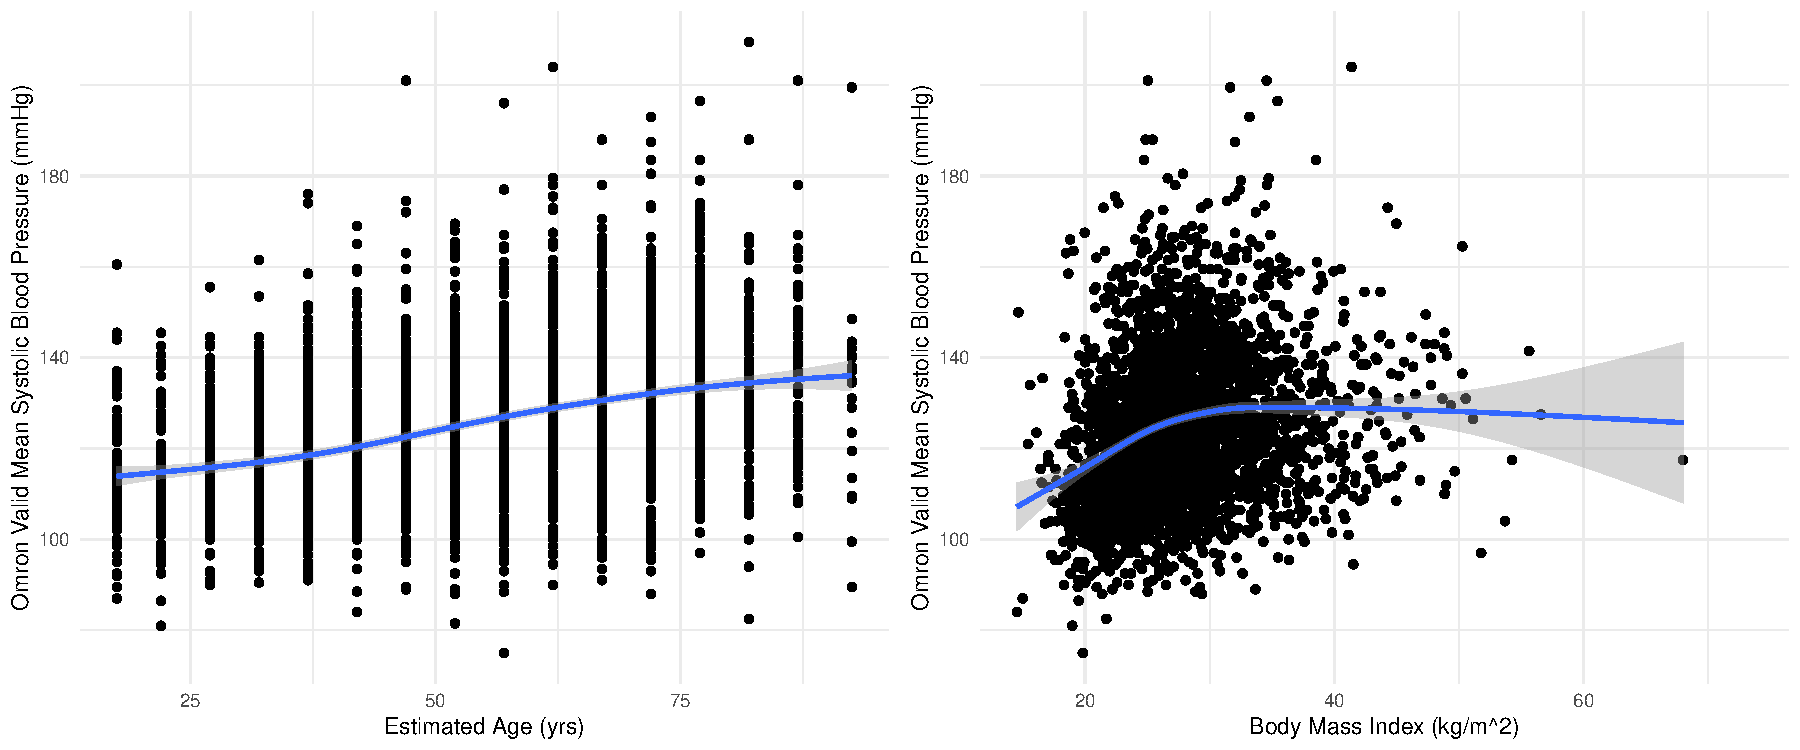
\includegraphics{Coursework_files/figure-latex/output-relationship-plots-1} \caption{Relationship of BMI and Age with Mean Systolic Blood Pressure}\label{fig:output-relationship-plots}
\end{figure}

To determine the predictors in the final model, we used a stepwise
approach starting with the full model and eliminating variables based on
AIC. The final model selected was \(MODEL\)

The Q-Q plot in Figure \ref{fig:output-qq-plot} shows a good fit to the
distribution and, despite some deviation at both ends of the scale, the
model can capture the outliers more accurately than other distributions
we tried. On our testing dataset we achieve a RMSE of 14.3mmHg, which is
relatively small compared to the threshold for hypertensive crisis of
140mmHg+.

\begin{figure}[H]

{\centering 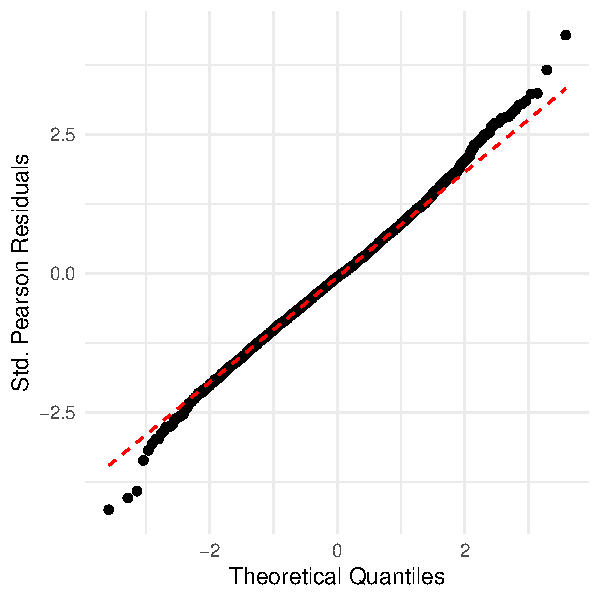
\includegraphics{Coursework_files/figure-latex/output-qq-plot-1} 

}

\caption{Q-Q plot of Inverse-Normal model residuals}\label{fig:output-qq-plot}
\end{figure}

We found that, on average, young females are predicted lower blood
pressure than young men but as they age, their blood pressure increases
at a faster rate. Controlling for other lifestyle choices included in
the model, a female's blood pressure can be expected to exceed an
equivalent male's at around 72 years old. Figure
\ref{fig:output-effect-plots-age} shows this relationship. One of the
biggest influences on BP was smoking status, and we found smoking was
associated with higher blood pressure for both males and females, also
shown in Figure \ref{fig:output-effect-plots}. This effect is largest
for males and a typical male can expect a 1.69\% increase in BP by
taking up smoking.

\begin{figure}[H]
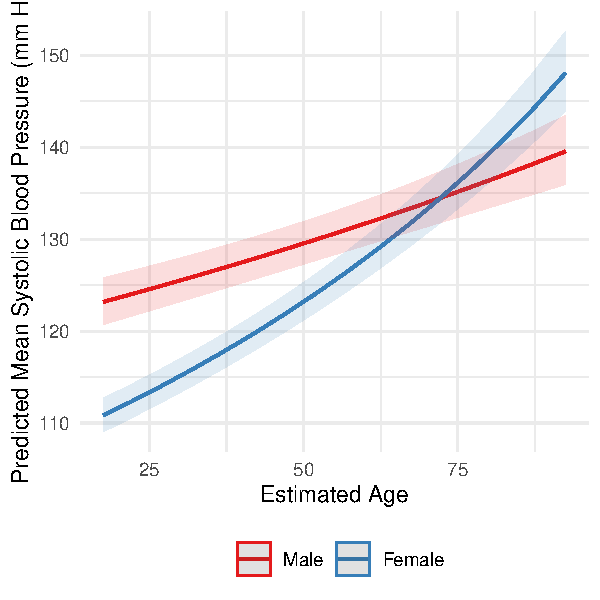
\includegraphics{Coursework_files/figure-latex/output-effect-plots-age-1} \caption{Marginal effects of Age on Systolic Blood Pressure}\label{fig:output-effect-plots-age}
\end{figure}

\begin{figure}[H]
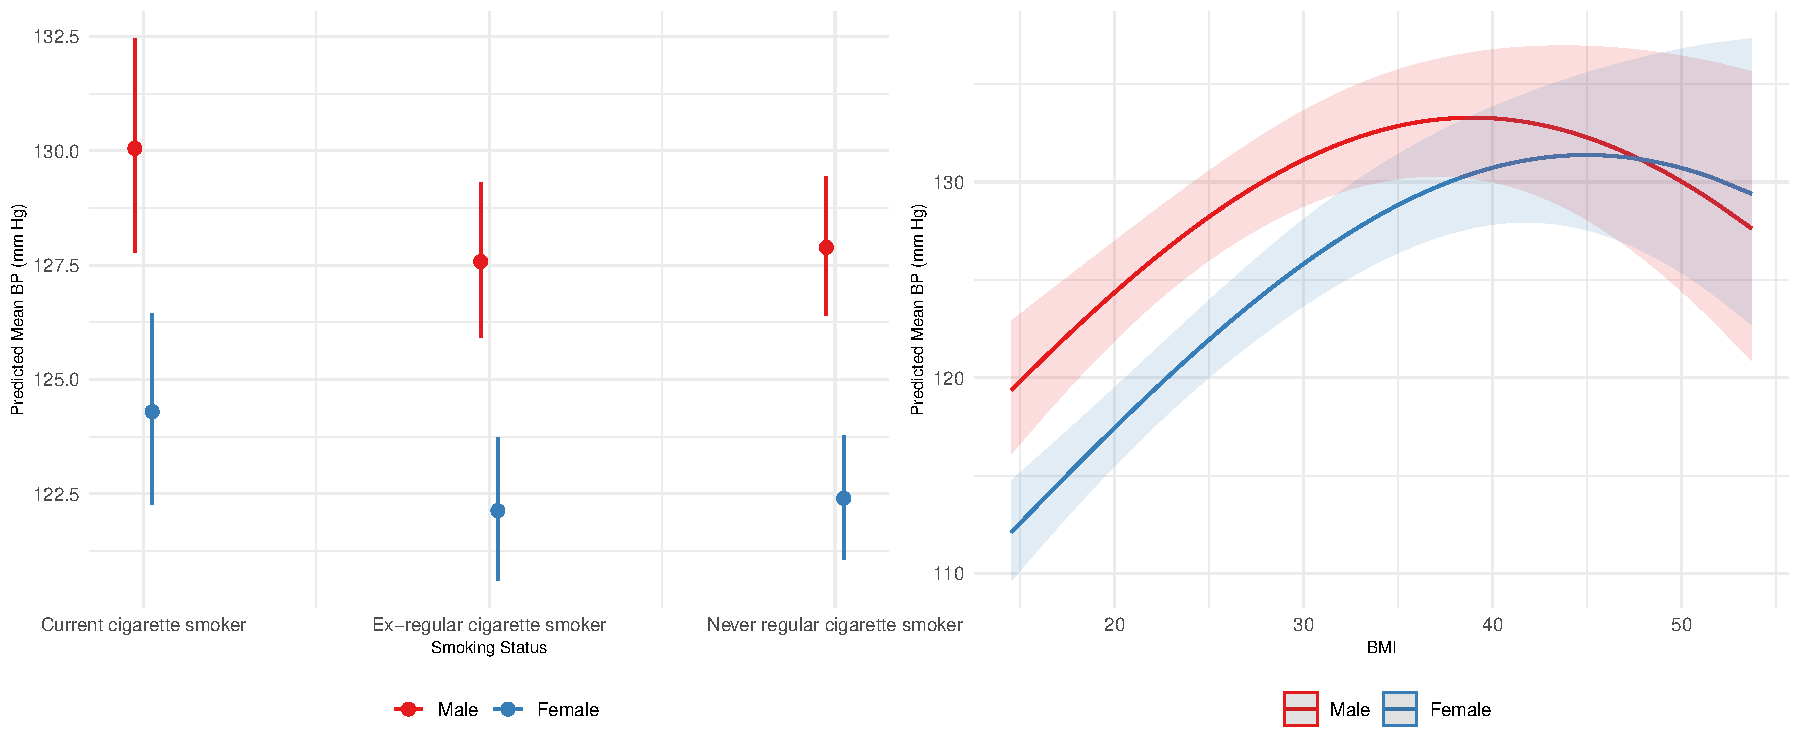
\includegraphics{Coursework_files/figure-latex/output-effect-plots-1} \caption{Marginal effects of Smoking Status and BMI on Systolic Blood Pressure}\label{fig:output-effect-plots}
\end{figure}

Drinking was also related to higher BP, and we observe a linear
relationship in Figure \ref{fig:output-effect-plots-alc} with the number
of days that alcohol was consumed in the previous week. On average, one
extra day of drinking led to an increase of 0.74 mmHg.

\begin{figure}[H]
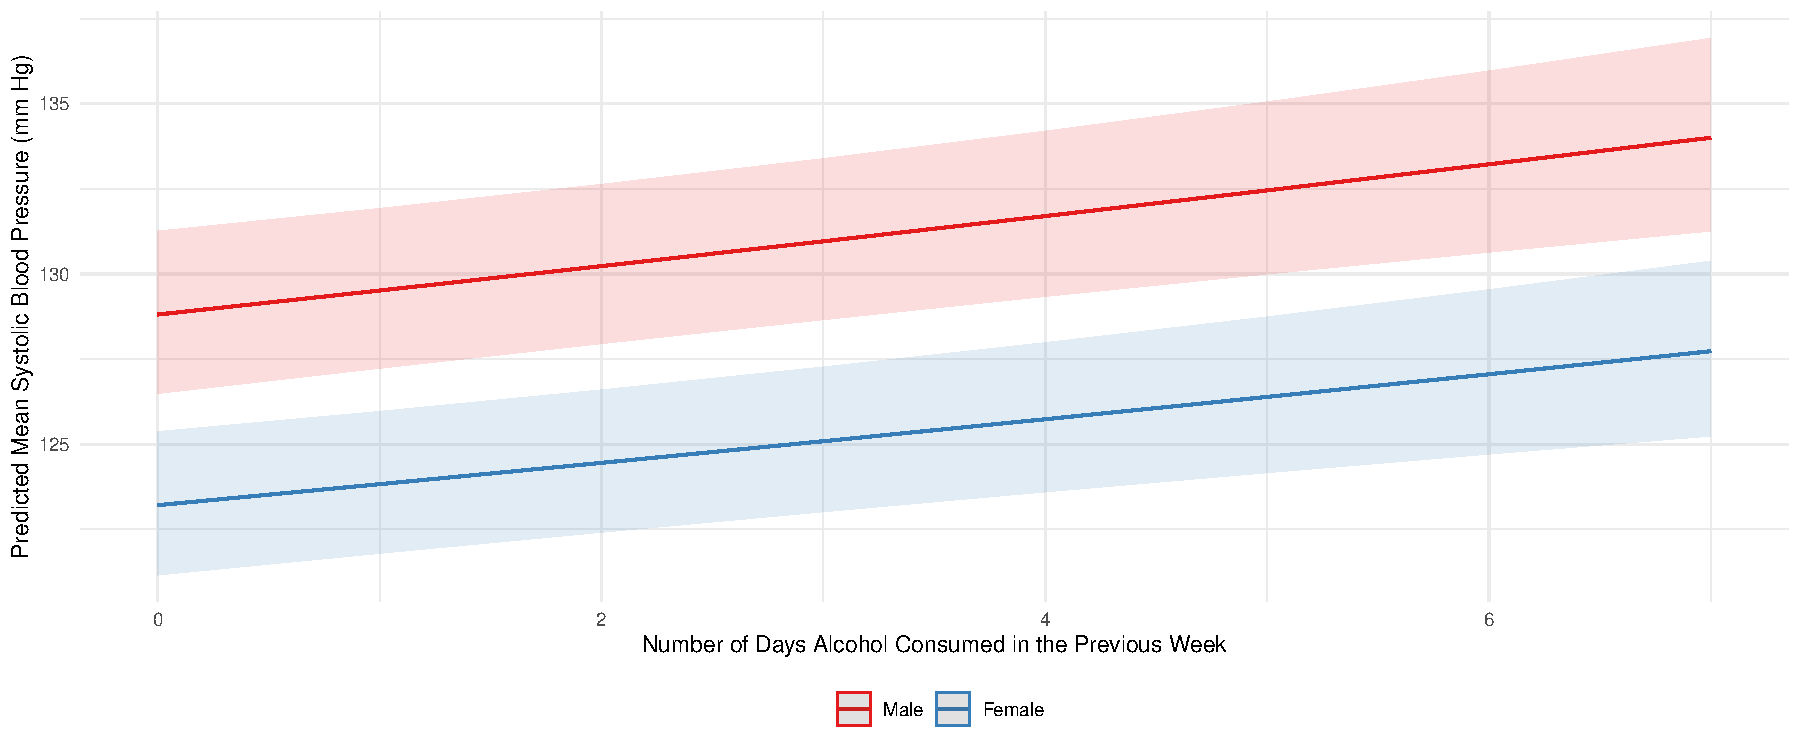
\includegraphics{Coursework_files/figure-latex/output-effect-plots-alc-1} \caption{Marginal effects of alcohol consumption on Systolic Blood Pressure}\label{fig:output-effect-plots-alc}
\end{figure}

\subsection{Results/Conclusion}\label{resultsconclusion}

Our analysis showed that alcohol consumption is extremely common among
UK adults, with approximately 80.4\% being consumers, while smoking and
vaping rates are lower at 16.5\% and 4.3\%, respectively. Older males
show the highest tendencies for alcohol consumption, with `frequent'
drinking the most prevalent among males aged 65-74. Unlike `frequent'
alcohol consumption, the prevalence of smoking decreases with age.
Individuals aged 16-24 appear to be the most susceptible to smoking
cigarettes, indicating a significant issue within youth culture.
Moreover, we found an interesting relationship between deprivation
levels and smoking and drinking behaviours. Smoking prevalence seemed to
increase as deprivation levels decrease, while alcohol consumption
appeared to do the opposite.

For interpretability, we decided to include a forest plot of the odds
ratio for each variable in our model, as the log-odds can be difficult
to interpret. Note, it is important to state the reference level of each
factor variable, so we have a baseline for comparison among other
levels. The intercept 0.257 can be interpreted as the probability of a
white, non-married, unqualified male living in urban area being a
smoker. On average, the blue factors increase the probability and the
red factors decrease the probability. Being Black, Asian, Married or a
female significantly decreases this probability.

To help us uncover the underlying socio-economic factors that may drive
the prevalence of smoking, we first looked at the most `comparable'
respondent type in our dataset. This `respondent' is a white, single
male who has no qualifications and lives in an urban area. We found that
the probability of our hypothetical respondent being a smoker is
approximately 25\%, which can be seen from Figure
\ref{fig:output-forest-plot}. This is notably higher than the population
average of 16.5. The smoking prevalence estimate in our sample is
significantly higher than the population of interest (16.5\% vs.~13.9\%,
outside of the CI in Table \ref{tab:output-estimates-table}). The only
socio-economic variables to certainly increase this probability is the
deprivation level our respondent falls under. The rest of the
socio-economic variables we have access to, appear to decrease the
likelihood of smoking. For example, if our respondent is any of the
following: Asian, black, married, or went on to further education, the
chances of them being a smoker is at-least halved.

\clearpage
\onecolumn

\section*{References}\label{references}
\addcontentsline{toc}{section}{References}

\phantomsection\label{refs}
\begin{CSLReferences}{1}{0}
\bibitem[\citeproctext]{ref-SexBMI}
al., Katsuya et. 2019. {``{The Investigation of Sex Differences in the
Effect of Body Mass Index}.''}
\url{https://www.hindawi.com/journals/ijhy/2019/1360328/}.

\bibitem[\citeproctext]{ref-AgeSex}
al., Martins et. 2019. {``{The effect of gender on age-related blood
pressure changes and the prevalence of isolated systolic hypertension
among older adults}.''} \url{https://pubmed.ncbi.nlm.nih.gov/11605350/}.

\bibitem[\citeproctext]{ref-SmokeCue}
Anastasia Droungas, Anna Rose Childress, Ronald N. Ehrman. 1995.
{``{Effect of smoking cues and cigarette availability on craving and
smoking behavior}.''}
\url{https://www.sciencedirect.com/science/article/pii/030646039500029C}.

\bibitem[\citeproctext]{ref-heart}
Association, American Heart. 2023. {``{Understanding Blood Pressure
Readings}.''}
\url{https://www.heart.org/en/health-topics/high-blood-pressure/understanding-blood-pressure-readings}.

\bibitem[\citeproctext]{ref-GovUK}
GOV.UK. 2014. {``{Tax on shopping and services}.''}
\url{https://www.gov.uk/tax-on-shopping/alcohol-tobacco}.

\bibitem[\citeproctext]{ref-DrinkCue}
Kambouropoulos, Nicolas. 2009. {``{{`Cue reward salience'} predicts
craving in response to alcohol cues}.''}
\url{https://www.sciencedirect.com/science/article/abs/pii/S0191886908003127}.

\bibitem[\citeproctext]{ref-AgeBMI}
Medicine, National Library of. 2017. {``{Weight and Body Mass Index in
Old Age: Do They Still Matter?}''}
\url{https://www.ncbi.nlm.nih.gov/pmc/articles/PMC5704942/}.

\bibitem[\citeproctext]{ref-Main}
NatCen Social Research, Department of Epidemiology, University College
London, and Public Health. 2019. {``{Health Survey for England}.''}
\url{http://doi.org/10.5255/UKDA-SN-8860-1}.

\bibitem[\citeproctext]{ref-1ONS}
ONS. 2019a. {``{Adult smoking habits in the UK: 2019}.''}
\url{https://shorturl.at/DMQXZ}.

\bibitem[\citeproctext]{ref-AccountPartner}
---------. 2019b. {``{Adult smoking habits in the UK: 2019}.''}
\url{https://shorturl.at/itPQU}.

\bibitem[\citeproctext]{ref-2ONS}
---------. 2019c. {``{Alcohol-specific deaths in the UK: registered in
2019}.''} \url{https://shorturl.at/gqxY1}.

\bibitem[\citeproctext]{ref-Deprivation}
---------. 2023. {``{Deprivation and the impact on smoking prevalence,
England and Wales: 2017 to 2021}.''} \url{https://shorturl.at/fuy48}.

\bibitem[\citeproctext]{ref-Omron}
Yechiam Ostchega PhD, Tatiana Nwankwo MS, RN. 2009. {``{Assessing the
Validity of the Omron HEM-907XL Oscillometric Blood Pressure Measurement
Device in a National Survey Environment}.''}
\url{https://onlinelibrary.wiley.com/doi/full/10.1111/j.1751-7176.2009.00199.x}.

\end{CSLReferences}

\end{document}
